%
% Thesis Style 用サンプル TeX
%
% コンパイルには llmk を用いること.
%
% 両面印刷する時は twoside にする
%
\documentclass[12pt,twoside]{jbook}
\usepackage{csg-thesis}
\usepackage[dvipdfmx]{graphicx}
\usepackage{url}
\usepackage{subcaption}

\begin{document}

% 題目
% 適当に改行(\\)で区切って見やすくする
\title{%
  Code Aile\\バーチャルペットを用いた\\プログラミング習慣化の試み
}

% 学位(学部と大学院で変更)
\degree{学士}
% \degree{修士}

% 名前
\author{%
  次原蒼司
}

% 提出日
\date{2024年2月7日}

% 卒業年度
\schoolyear{2025年}

% 所属(学部と大学院で変更)
% \department{京都産業大学 コンピュータ理工学部 コンピュータサイエンス学科}
% \department{京都産業大学 コンピュータ理工学部 ネットワークメディア学科}
% \department{京都産業大学 コンピュータ理工学部 インテリジェントシステム学科}
\department{京都産業大学 情報理工学部}
% \department{京都産業大学大学院 先端情報学専攻}

% 学籍番号
\stnumber{2153939}

% 指導教員(教官ではなくなった...)
\supervisor{玉田 春昭}

\pagenumbering{roman}  %% ページ番号をローマ数字にする

\maketitle

%%%%%%%%%%%%%%%%%%%%%%%%%%%%%%%%%%%%%%%%%%%%%%%%%%%%%%%%%%%%%%%%%%%%%%

% 概要
\begin{abstract}
 プログラミング初学者の多くは、その好き嫌いや得意不得意に関わらず、習慣的にプログラミング開発を継続することが難しいという課題がある。
この課題を解決するためには、当人の努力や意志に頼らず、習慣化を促すための動機付けが必要である。
そこで本稿ではその動機付けの一環として、ペット育成ゲームの要素を取り入れたゲームを考え、
それを今日デファクト・スタンダードな統合開発環境/IDEであるVSCodeに実装した拡張機能、Code Aileを提案する。
用意された実績を解除し、ペットを育てるという要素を取り入れることで、開発の達成感を高め、ユーザーのモチベーション維持に繋げる。
試験的に本拡張機能を使用したユーザーにアンケートを行い、その結果から本拡張機能の有効性を検証する。
実験の結果、バーチャルペットを育てることはプログラミング習慣化の手助けになることが分かった。
しかし、Code Aileという拡張機能のシステムやUIには改善が必要であるという結論になった。

\end{abstract}

% 謝辞
\begin{acknowledgments}
% ちょっとくだけすぎかも
本稿は以下の方々なくして、存在しえなかったでしょう。
研究に対する助言や資料の提供など指導していただいた玉田春昭教授、
並びに研究や成果物の評価に協力していただいた研究室の皆さん。
心より感謝しています。

\end{acknowledgments}

%%%%%%%%%%%%%%%%%%%%%%%%%%%%%%%%%%%%%%%%%%%%%%%%%%%%%%%%%%%%%%%%%%%%%%

\tableofcontents       %% 目次

%
% 目次等にはローマ数字を使い、本文開始ページを 1 ページ目にできる
% この方が見た目がきれいであるが、全体のページ数は減って見える
% ここでローマ数字に変えた場合は chapter 1 でアラビア数字に戻すこと
%

\listoffigures         %% 図目次(図がない場合は不要)
\listoftables          %% 表目次(表がない場合は不要)

%%%%%%%%%%%%%%%%%%%%%%%%%%%%%%%%%%%%%%%%%%%%%%%%%%%%%%%%%%%%%%%%%%%%%%

\pagenumbering{arabic}
%
% 本文
%
\chapter{はじめに}

 プログラミングに限らず、学習には継続的な努力が必要であり、そのためには継続する動機が必要である。
そのためにこれまで、ゲーミフィケーション\cite{2022caeai_zhan}やエディテインメント\cite{2020ipsj_hanayama}に基づく手法が提案されてきた。
これらは、ゲームや娯楽を通じて学習を促進する手法であり、プログラミング教育においても、
プログラミング言語の学習をゲーム感覚で行うことで、学習意欲を高める取り組みが行われている\cite{2014hicss_hamari}。

 そこで本稿では、ゲーミフィケーションを取り入れたVSCode 拡張機能を開発する。
VSCode は現在最も普及しているエディタであり、ユーザーが非常に多い。
それにより、初学者が開発に対するモチベーションを維持できるような環境構築を目指す。
具体的には、キャラクターを成長させることができる育成ゲームの要素を取り入れ、
ユーザーの進捗を視覚的にフィードバックするため、サイドバーを部屋に見立てて育成するキャラクターを配置する。
そしてユーザーは、開発を行うことで実績を解除し、経験値を得てキャラクターを成長させる。この実績システムでは、ソース
ファイルの新規作成数や編集行数、デバッグ回数などを追跡し、これらの操作をもとに実績を解除できる。
このシステムによってユーザーにフィードバックと達成感を与え、さらなる開発への動機付けになると考えられる。
また、達成した実績数に応じて、部屋に飾るアイテムを取得することができる。これによりユーザーは、
単なる学習成果のみならず、キャラクターの成長や部屋のカスタマイズといった要素を楽しみながら、自主的に開発を継続できると期待できる。
これらを通じて、プログラミング初学者が日常的にコーディングを続けられる環境を提供し、モチベーションの維持と開発習慣の定着を目指す。

%%%%
\chapter{提案手法} \label{sec:proposal}

 本稿では、初学者が楽しみながらプログラミング開発を習慣化できるような環境を提供することを目的とする。
そのために、広く使用されているエディタであるVisual Studio Code(VSCode)に対して、
ゲーミフィケーション要素を取り入れた拡張機能を提供する。

 本拡張機能が満たすべき要件は以下の3つである。
\begin{quote}
	\begin{enumerate}
	 \item インストールが容易であること
	 \item 利用方法が直感的であること
	 \item 開発を継続できる仕組みがあること
	\end{enumerate}
\end{quote}

 要件1は、拡張機能の利用者が初学者であることを想定しているため、アカウント作成や環境構築など、
利用開始に余計な手間を要しない事が重要である。VSCodeでは一般的な拡張機能と同様に、
Visual Studio Marketplaceで提供可能であるため、この要件を満たせると考えられる。

 要件2は、初学者が簡単に機能を利用できることを意味する。そのため、本拡張機能ではユーザーが操作可能なインターフェースは最小限に抑える。
具体的には、キャラクターを進化させるボタンと進捗を表示するボタンの2つのみを提供する。
これによりユーザーは、基本的には画面上で成長するキャラクターを眺めるだけであり、操作に迷うことなく直感的に利用できるため、この要件も満たせると考えられる。

 要件3は、開発の継続を促進させる仕組みを持つことである。これを実現するために、本拡張機能には実績システムを導入する。
ユーザーが開発を行う中で一定の条件を満たすと、実績が解除される仕組みとし、
解除時にユーザーにフィードバックと達成感を与えることで、ユーザーのモチベーション向上と開発の継続を促す。
このシステムの導入により、要件3は満たせると考えられる。

% 引用の例
% Javassist\cite{2000ecoop_chiba,2003gpce_chiba}は...
% Javassistは\cite{javassist}で配布されている。

%%%%
\chapter{実装}
 これまでに述べた内容を基に、TypeScriptおよびVSCode APIを用いて、プログラミング習慣化のためのVSCode拡張機能Code Aileを作成した。
Code Aileは、VSCodeのサイドバーに表示される部屋を舞台に、キャラクター(Aile)を成長させたり、Aileの部屋をカスタマイズする機能を提供している。
また、Aileの成長や部屋のカスタマイズ機能は、第\ref{sec:proposal}章で述べた実績システムと連動しており、
そのためにVSCodeを通じて、ファイルの新規作成、保存、編集行数、デバッグの実行などユーザーの操作を追跡する機能も実装している。

\section{Aileの成長と部屋のカスタマイズ}
 Aileの成長段階は7段階あり、ユーザーランクと連動して成長する。
実行画面にあるevolve aile(EA)ボタンをクリックすることで、Aileが次の成長段階に進化する。
また、解除した実績数が5つ増えるごとに、部屋のカスタマイズアイテムを取得でき、部屋の背景を変更したり、家具を配置することができる。
図~\ref{fig:initialCodeAile}が、初期段階の実行画面であり、図~\ref{fig:grownCodeAile}は、ある程度成長した段階の実行画面である。

\begin{figure*}[t]
	\begin{minipage}[b]{0.48\linewidth}
		\centering
		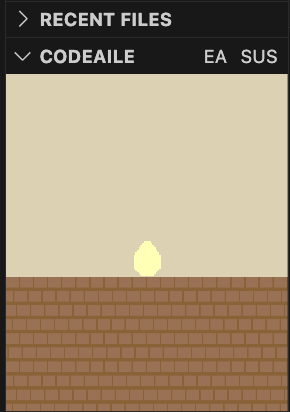
\includegraphics[width=4cm]{images/initialCodeAile}
		\subcaption{CodeAileの実行画面(初期段階)}
		\label{fig:initialCodeAile}
	\end{minipage}
	\hfill
	\begin{minipage}[b]{0.48\linewidth}
		\centering
		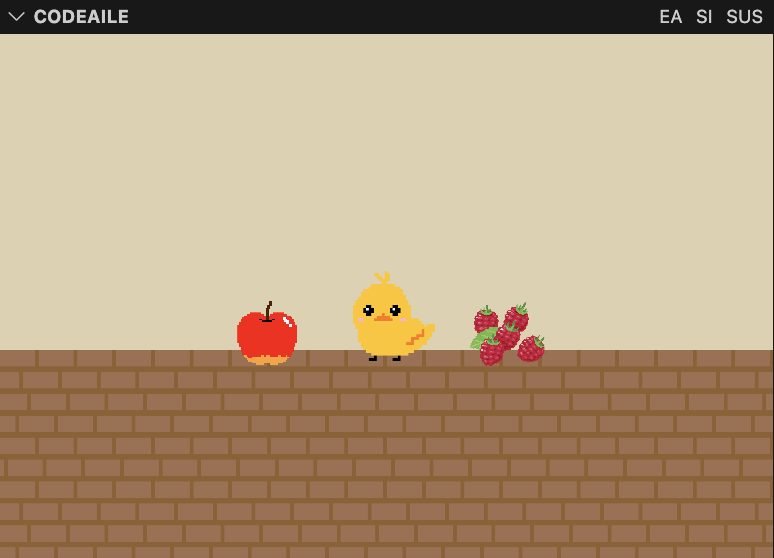
\includegraphics[width=4cm]{images/grownCodeAile}
		\subcaption{CodeAileの実行画面(成長後)}
		\label{fig:grownCodeAile}
	\end{minipage}
	\hfill
	\caption{CodeAileの実行画面}
	\label{fig:codeAile}
\end{figure*}

\section{ユーザーステータス}
 ユーザーステータスはユーザー名、経験値、ランク、解除した実績リストの4要素を持つ。
ユーザー名はホームディレクトリ名が自動的に設定され、実績を解除することで経験値が増加し、次のランクに上がるための閾値に達するとランクが上昇する。
実行画面にあるshow status(SS)ボタンをクリックすることで、図\ref{fig:userStatus}の様に、現在のステータスと実績の達成状況を確認できる。

\begin{figure}[tb]
  \centering
  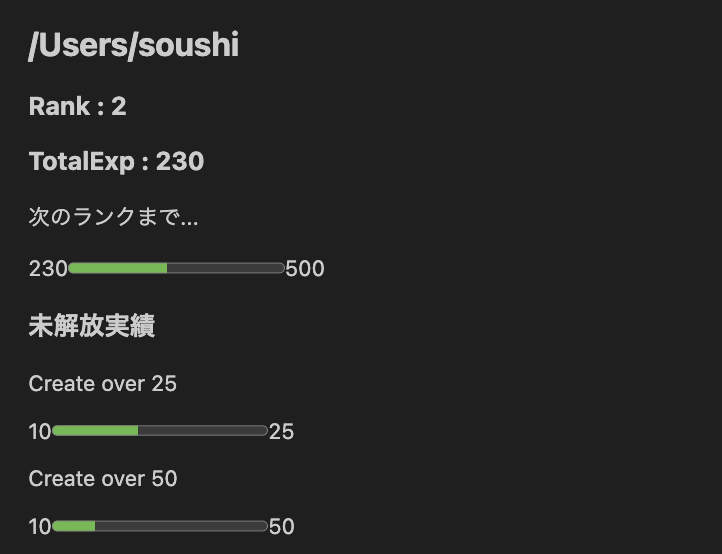
\includegraphics[width=10cm]{images/userStatus}
  \caption{ユーザーステータスの表示}
  \label{fig:userStatus}
\end{figure}

\section{実績システム}
 ログファイルから得た統計情報を取得し、事前に設定している実績の条件を満たしていると、実績が解除される。
条件は10種類あり、それぞれ難易度が5段階の、計50個の実績とそれに応じて得られる経験値が設定されている。

\section{ログシステム}
 VSCode APIを用いて、VSCode上での以下の操作を追跡し、それをログファイル($HOME/.config/codeaile/logfile.txt)に記録する。
 これらの操作はユーザーが開発を行う中での主要な操作であり、これによりユーザーの開発状況を把握し、実績システムに活用することができる。
\begin{quote}
  \begin{itemize}
   \item ファイルの新規作成(Create)
   \item ファイルをエディタで開く(Open)
   \item ファイルを保存する(Save)
   \item ファイルの編集行数(ChangeLineCount)
   \item デバッグの実行(Debug)
   \item VSCodeがアクティブであるか(FocusIn/Out)
  \end{itemize}
\end{quote}

 また、ログファイルのフォーマットは図~\ref{fig:aileLog}の様になっており、VSCode実行中に定期的(1回/5分程度)に確認し、
図\ref{fig:statistics}の様に、編集行数やデバッグの実行回数などの統計情報を抽出する($HOME/.config/codeaile/statistics-data.txt)。

\begin{figure}[tb]
  \centering
  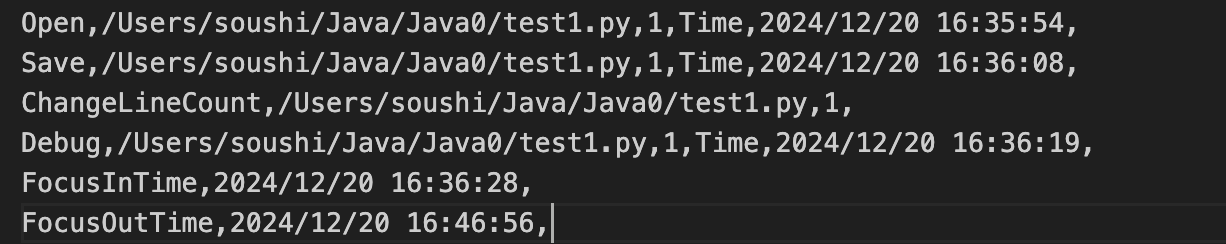
\includegraphics[width=10cm]{images/aileLog}
  \caption{ログファイルの一部}
  \label{fig:aileLog}
\end{figure}

\begin{figure}[tb]
  \centering
  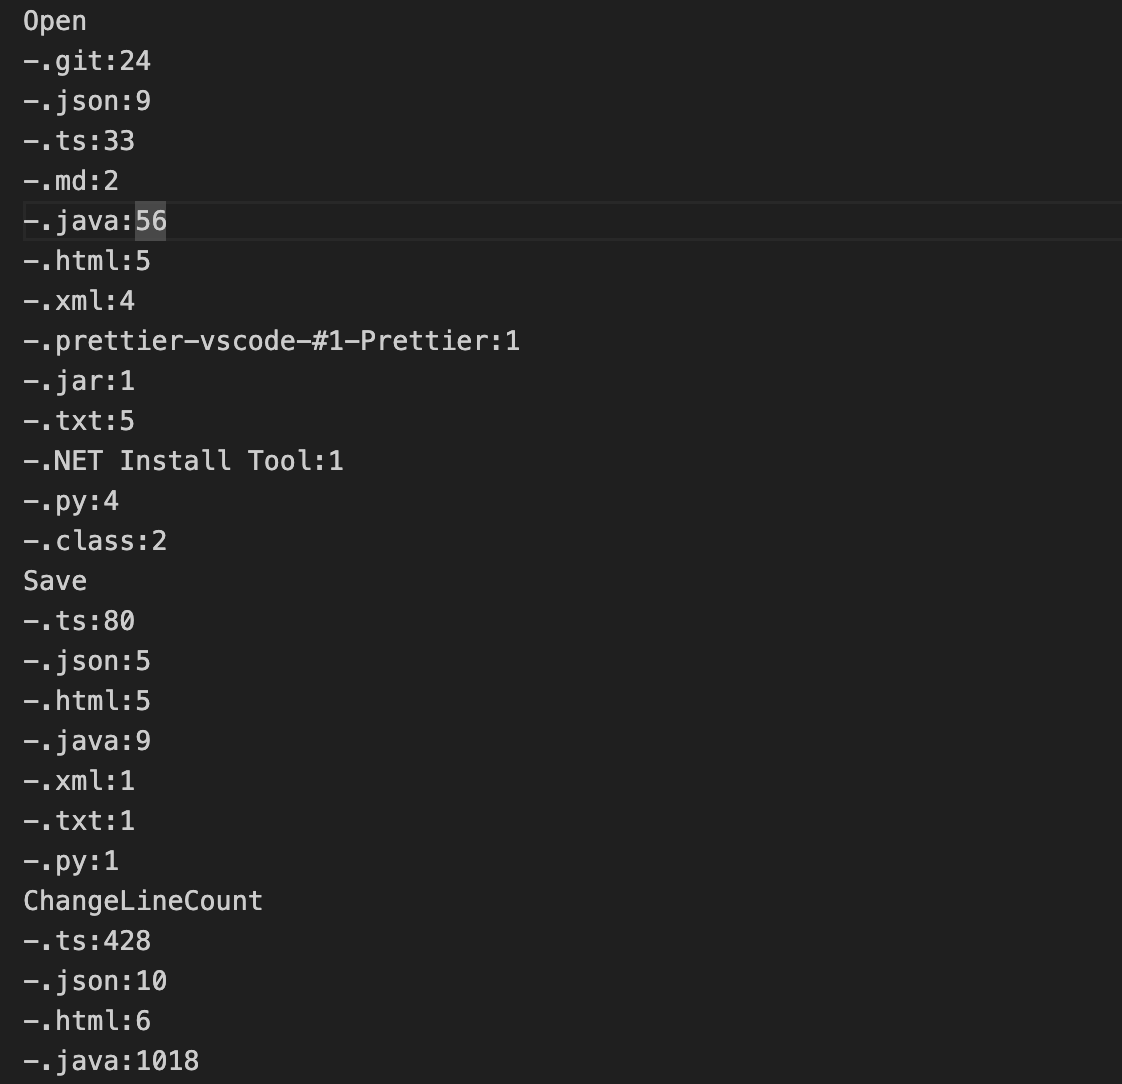
\includegraphics[width=10cm]{images/statistics}
  \caption{ログの統計データの一部}
  \label{fig:statistics}
\end{figure}

% % 図の例
% \begin{figure}[tb]
%   \centering
%   \includegraphics[width=10cm]{javassist.eps}
%   \caption{Javassistの処理の流れ}
%   \label{fig:javassist}
% \end{figure}

% 図~\ref{fig:javassist}は...

%%%%
\chapter{評価実験}

\section{実験手順}
 この拡張機能が実際にプログラミング開発の習慣化に貢献するか確かめるために、実験参加者を募り、評価実験を行った。
実験参加者にはCode Aileを2週間に渡り使用させ、その後アンケート調査を行った。
アンケートの内容は、以下の通りである。
\begin{quote}
	\begin{enumerate}
    % \item 現在の経験値総量・ランクを教えてください。
    % \item 総ログイン日数・連続ログイン日数を教えてください。
    \item プログラミング開発を楽しむことができましたか。
    \item 実績を解除すること、Aileを育てることは、プログラミング開発のモチベーションになりましたか。
    \item これからも開発を継続しようと思いましたか。
    \item 開発を継続しようと思った人は、これからもCode Aileを使用しようと思いますか。
    \item Code Aileを初学者に勧めたいと思いましたか。
    \item この機能の良かった点があれば教えてください。
    \item この機能の悪かった点があれば教えてください。
    \item その他、感想や要望があれば教えてください。
	\end{enumerate}
\end{quote}

\section{実験結果}
 図~\ref{fig:q1}〜図~\ref{fig:q5}より、プログラミング開発を楽しめた人は実験参加者の半数であり、
同じく半数の人が、Aileの存在がモチベーションに繋がったと回答している。また、開発を継続しようと思った人は過半数を超えており、
同様に過半数の人がCode Aileを今後も利用したい、Code Aileを初学者に勧めたいと回答している。
この結果は、初学者の学習支援を目的としたCode Aileにとって、良い結果だと言える。
 図~\ref{fig:q6}の回答より、良かった点としてキャラクターの成長と自分の成長を一緒に実感できる、学習の進捗が視覚的に分かる等、
Code Aileの狙いである、視覚的フィードバックによるモチベーションの向上が、実現できていると考えられる。
 ただし、図~\ref{fig:q7}、図~\ref{fig:q8}の回答のように、悪かった点も多く挙げられており、
ボタンを押すことでAileが進化するというシステムの都合上、コードを編集している時にはAileの変化がなくモチベーションが湧かない、
ランクがいつ・どのように上がったのか分からないといったシステム面、その他ステータス通知が邪魔になる、Aileを手動で進化させなければならない、
などUI面での意見をいただいた。これらの意見より、ランクアップしたことが分かる通知機能や、Aileが自動で進化する様な仕組み、
Aileのアイテムや進化条件がわかりやすくなるようなUIの改善が必要だと考えられる。

% \begin{table*}[t]
% 	\caption{経験値総量・ランク・総ログイン日数・連続ログイン日数をまとめた表}
% 	\label{log}
% 	\center
% 	\includegraphics[height=6cm]{images/log}
% \end{table*}

\begin{figure*}[t]
  \hfill
  \begin{minipage}[b]{0.48\linewidth}
    \centering
    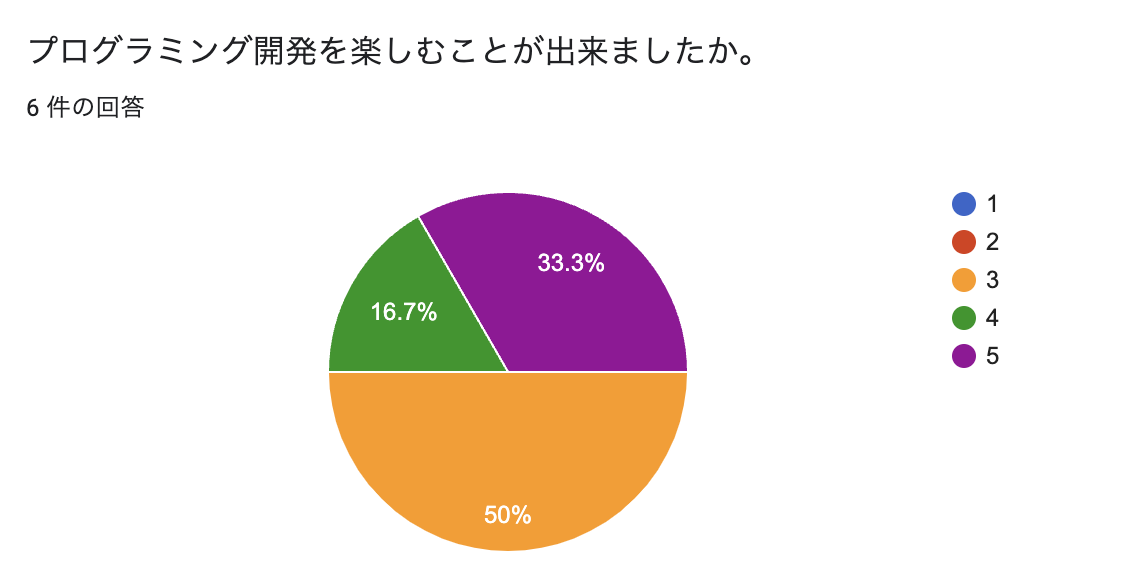
\includegraphics[width=4cm]{images/q1}
    \caption{質問1への回答}
    \label{fig:q1}
  \end{minipage}
  \hfill
  \begin{minipage}[b]{0.48\linewidth}
    \centering
    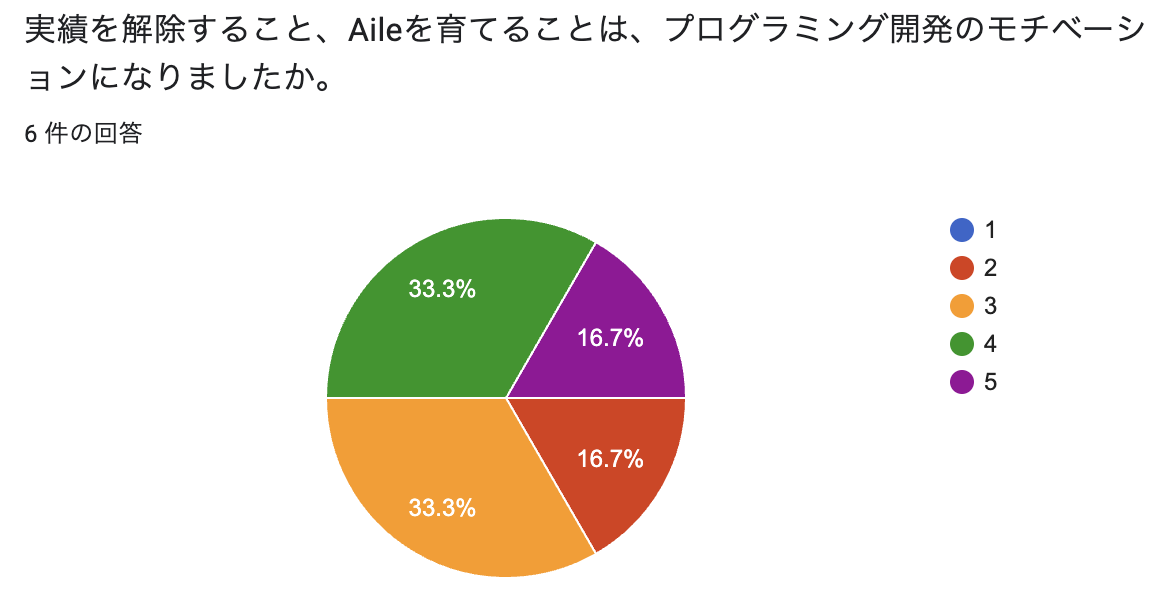
\includegraphics[width=4cm]{images/q2}
    \caption{質問2への回答}
    \label{fig:q2}
  \end{minipage}
  \hfill
  \begin{minipage}[b]{0.48\linewidth}
    \centering
    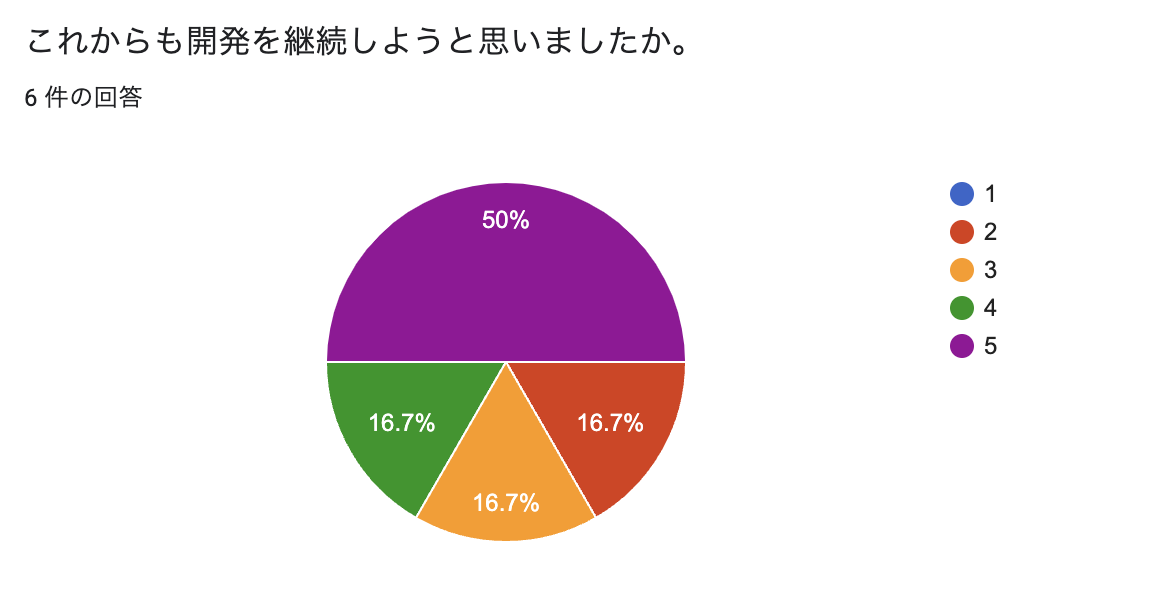
\includegraphics[width=4cm]{images/q3}
    \caption{質問3への回答}
    \label{fig:q3}
  \end{minipage}
  \hfill
  \begin{minipage}[b]{0.48\linewidth}
    \centering
    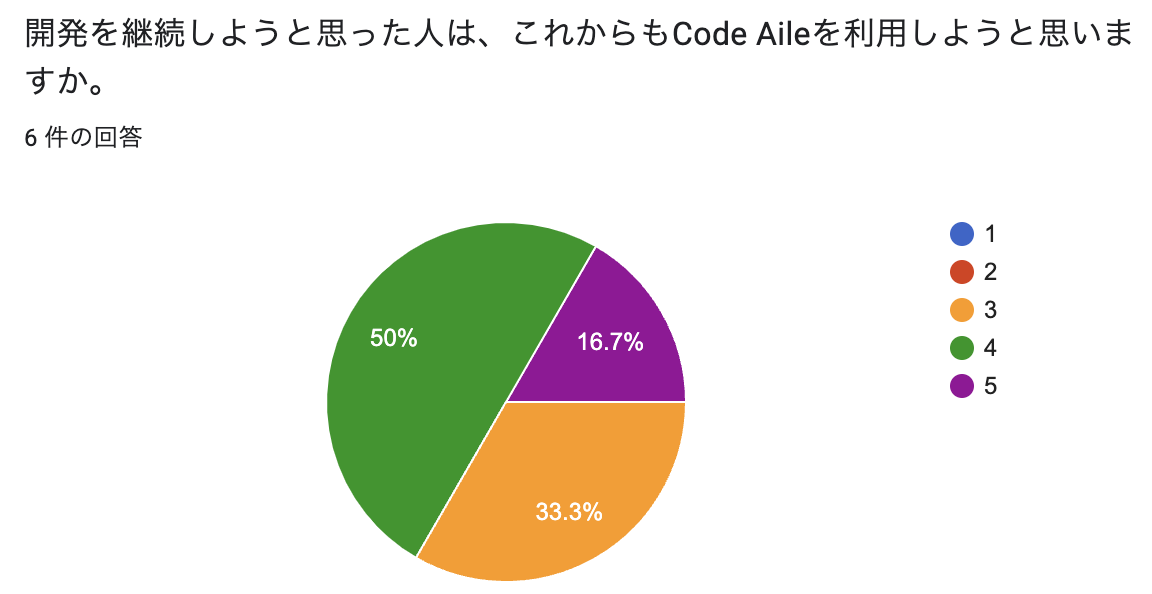
\includegraphics[width=4cm]{images/q4}
    \caption{質問4への回答}
    \label{fig:q4}
  \end{minipage}
  \hfill
  \begin{minipage}[b]{0.48\linewidth}
    \centering
    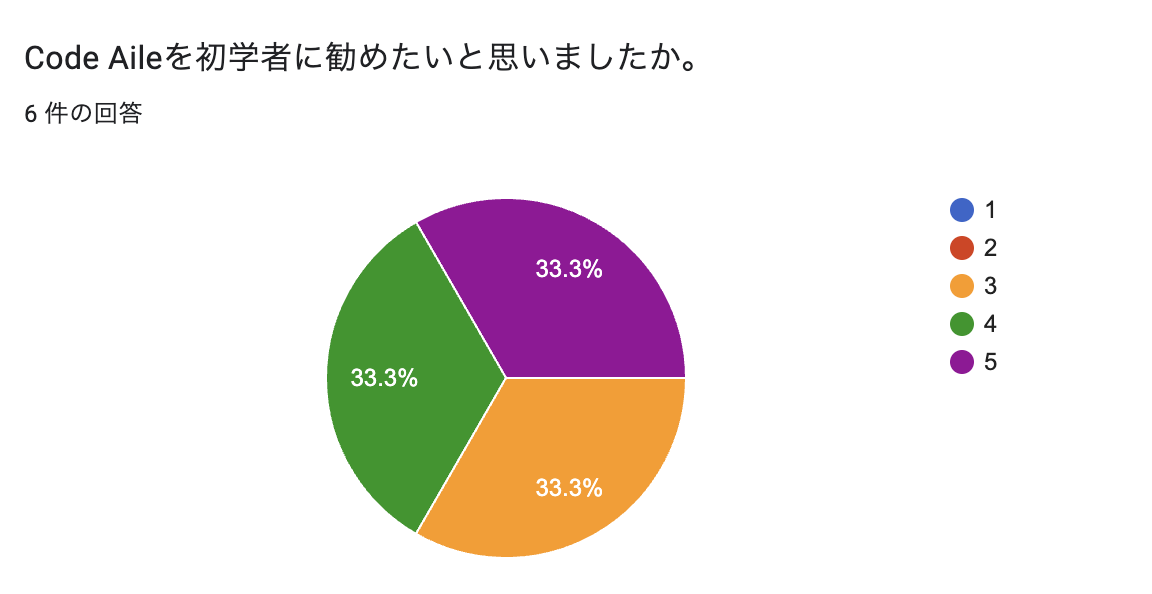
\includegraphics[width=4cm]{images/q5}
    \caption{質問5への回答}
    \label{fig:q5}
  \end{minipage}
  \hfill
  \begin{minipage}[b]{0.48\linewidth}
    \centering
    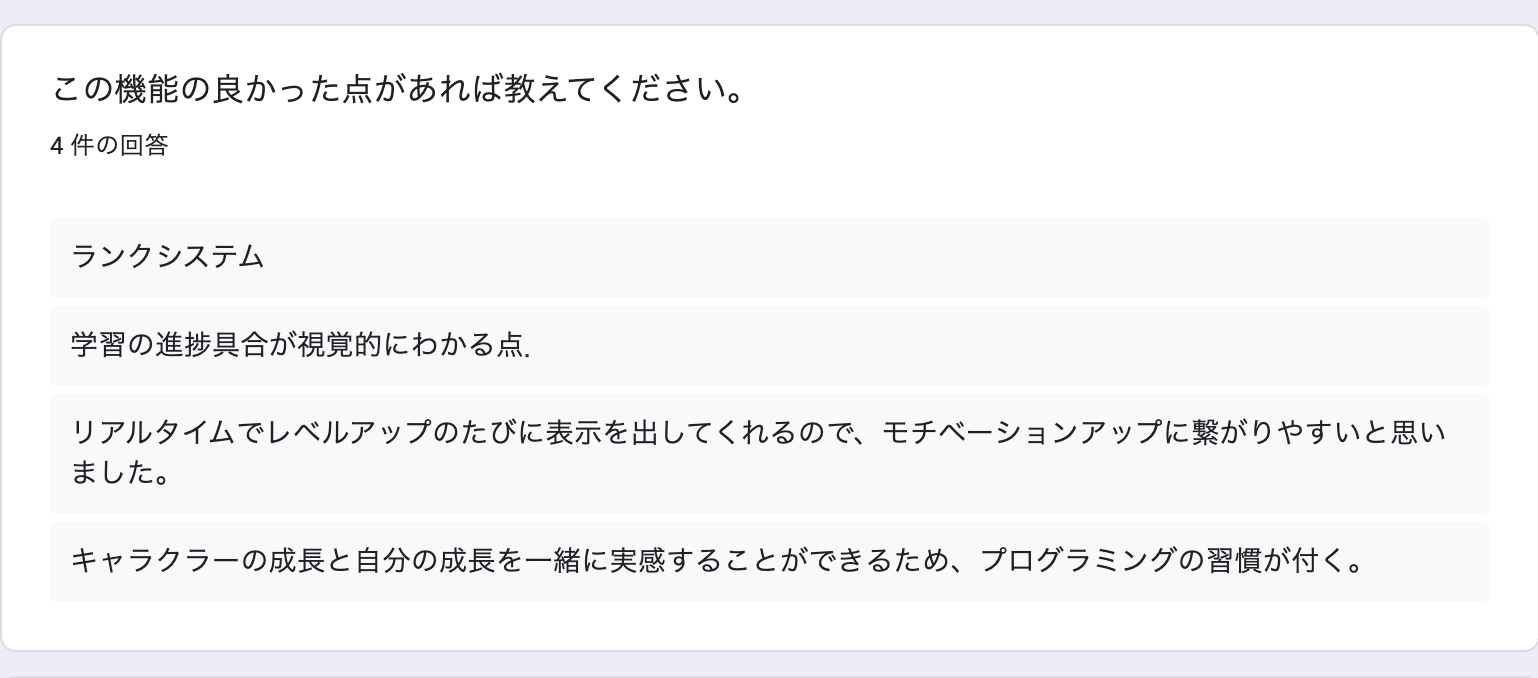
\includegraphics[width=4cm]{images/q6}
    \caption{質問6への回答}
    \label{fig:q6}
  \end{minipage}
  \hfill
  \begin{minipage}[b]{0.48\linewidth}
    \centering
    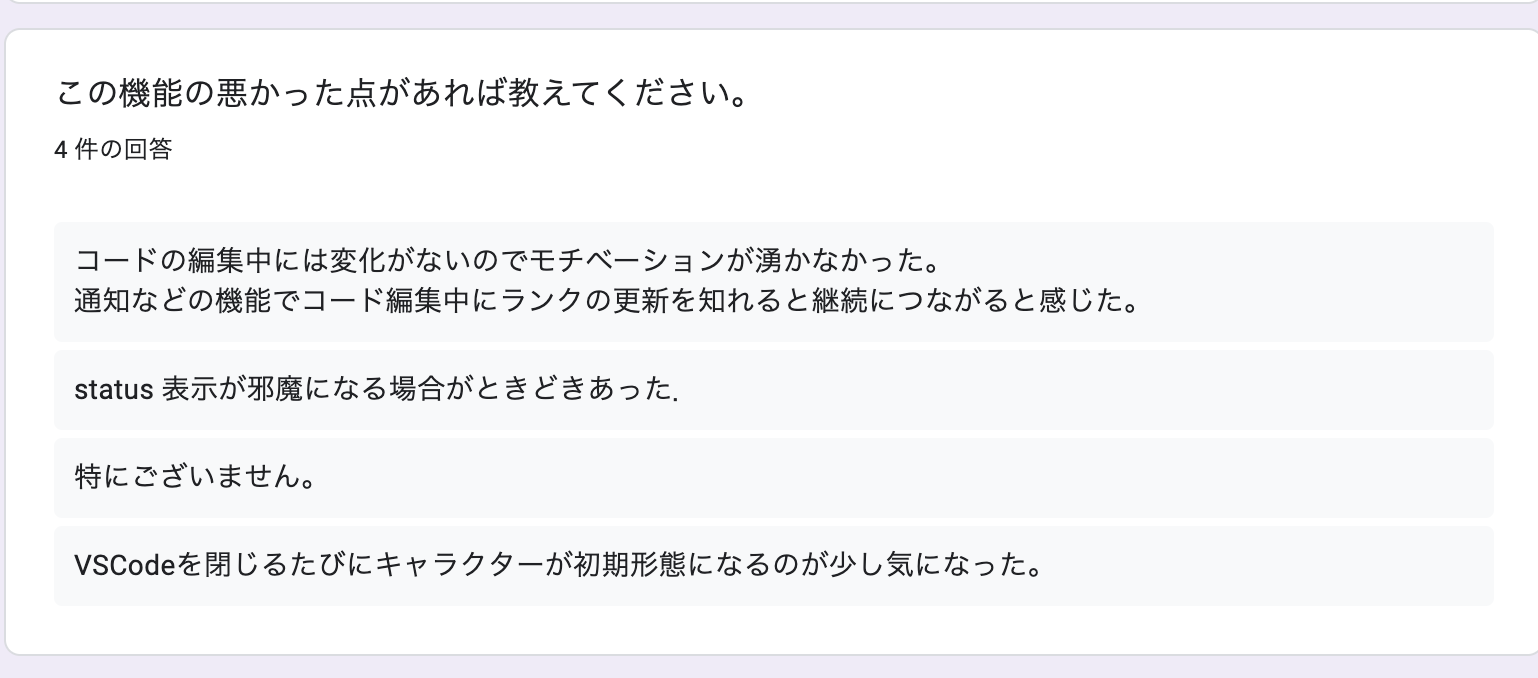
\includegraphics[width=4cm]{images/q7}
    \caption{質問7への回答}
    \label{fig:q7}
  \end{minipage}
  \hfill
  \begin{minipage}[b]{0.48\linewidth}
    \centering
    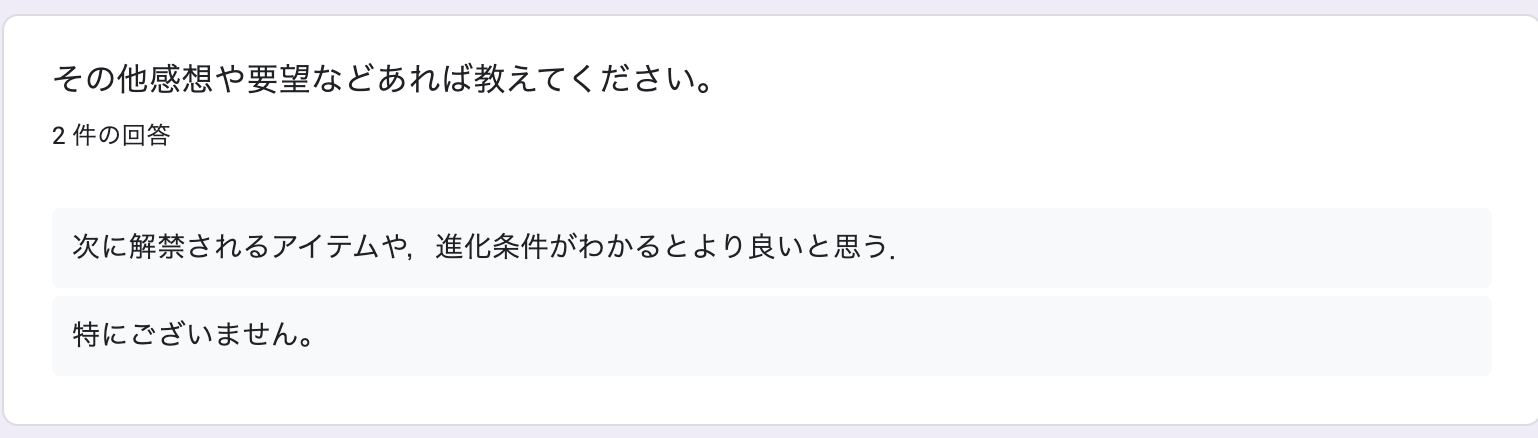
\includegraphics[width=4cm]{images/q8}
    \caption{質問8への回答}
    \label{fig:q8}
  \end{minipage}
  \hfill
  \caption{Code Aileの利用者アンケート結果}
  \label{fig:results}
\end{figure*}

%%%%
\chapter{まとめ}
 初学者がプログラミング開発を習慣化するために、バーチャルペットを育成と実績システムを用いたVSCode拡張機能、Code Aileを提案、実装した。
Code Aileの効果をアンケートで評価実験を行った結果、バーチャルペットを育成することは、プログラミング開発を継続するモチベーションになることが分かった。
それと同時に、Code AileのシステムやUIには改善が必要であるという結論になった。この実験結果より、プログラミング開発を習慣化するためには、
バーチャルペットの育成の様な視覚的フィードバックの他に、次のステップへ進むための目標掲示を行うなど、
ユーザーのモチベーションを維持する工夫がさらに必要であることが分かった。
今回、Code Aileの利用によってある程度習慣化を促すことが出来たが、これをより良い機能とするために追加で必要な要素が明らかになった。

%%%%%%%%%%%%%%%%%%%%%%%%%%%%%%%%%%%%%%%%%%%%%%%%%%%%%%%%%%%%%%%%%%%%%%

%
% 参考文献は直接書いてもいいが、bibtex を使うと便利
%  (1)このサンプルを platex にかける
%  (2)jbibtex thesis
%  (3)さらに platex にかける
%  (4)もう何回か platex にかける
%
\bibliographystyle{csg-thesis}
\bibliography{thesis.bib}

%%%%%%%%%%%%%%%%%%%%%%%%%%%%%%%%%%%%%%%%%%%%%%%%%%%%%%%%%%%%%%%%%%%%%%

% 付録が必要ならつける
\appendix
% \chapter{プログラム例}


\end{document}
